\documentclass[letterpaper, reqno,11pt]{article}
\usepackage[margin=1.0in]{geometry}
\usepackage{color,latexsym,amsmath,amssymb,graphicx, float}
\usepackage{hyperref}

\hypersetup{
colorlinks=true,
linkcolor=magenta,
filecolor=magenta,
urlcolor=cyan,
}

\graphicspath{ {images/} }

\begin{document}
\pagenumbering{arabic}
\title{PHYS 304 Homework 3}
\date{02/02/22}
\author{Xander Naumenko}
\maketitle

{\noindent\bf Question 1.} 
\[
\left<x \right>=\int \psi_n^* x\psi_n dx=\int_0^a \frac{2}{a}x\sin^2\left( n\frac{\pi}{a}x \right)dx=\int_0^a \frac{1}{a}x\left(1-\cos\left( \frac{2n\pi}{a}x \right)\right)dx
\]
\[
=\frac{a}{2}+\frac{-x\sin\left( \frac{2n\pi}{a}x \right) }{2n\pi}\bigg|_0^a+\int_0^a \frac{1}{2n\pi}\sin\left( \frac{2n\pi}{a}x \right) dx=\frac{a}{2}
.\]

\[
\left<x^2 \right>=\int \psi_n^* x^2\psi_n dx=\int \frac{2}{a}x^2\sin^2\left( n\frac{\pi}{a}x \right)dx=\int_0^a \frac{1}{a}x^2\left(1-\cos\left( \frac{2n\pi}{a}x \right)\right)dx
\]
\[
=\frac{1}{3}a^2+\frac{-x^2\sin\left( \frac{2n\pi}{a}x \right) }{2n\pi}\bigg|_0^{a}+\int_0^a \frac{x}{n\pi}\sin\left( \frac{2n\pi}{a}x \right) dx
\]
\[
=\frac{1}{3}a^2-\frac{xa\cos\left( \frac{2n\pi}{a}x \right) }{2n^2\pi^2}\bigg|_0^a+\int_0^{a}\frac{a\cos\left( \frac{2n\pi}{a}x \right) }{2n^2\pi^2}dx=\frac{1}{3}a^2-\frac{a^2}{2n^2\pi^2}
.\]

\[
\left<p \right>=m \frac{d\left<x \right>}{dt}=0
.\]

\[
\left<p^2 \right>=\int \psi_n^* \left(-\hbar^2 \frac{\partial^2}{\partial x^2}\right)\psi_n dx=\int_0^a \frac{2}{a}\frac{n^2\pi^2 \hbar^2}{a^2}\sin^2\left( \frac{n\pi}{a}x \right) dx=\frac{n^2\pi^2\hbar^2}{a^2}
.\]

\[
\sigma_x=\sqrt{\left<x^2 \right>-\left<x \right>^2}=\sqrt{\frac{1}{12}a^2-\frac{a^2}{2n^2\pi^2}}  
.\]

\[
\sigma_p=\sqrt{\left<p^2 \right>-\left<p \right>^2} =\frac{n\pi\hbar}{a}
.\]

\[
\implies\sigma_x\sigma_p=\sqrt{\frac{1}{12}a^2-\frac{a^2}{2n^2\pi^2}}  \frac{n\pi\hbar}{a}\geq \frac{\hbar}{2}
.\]
As expected the product of their standard deviations obeys the uncertainty principle. 

{\noindent\bf Question 2.} For the case that the potential is zero between $0$ and $2a$, we know thatthe solutions are of the form

\[
\psi_n(x)=\sqrt{\frac{2}{2a}} \sin\left( \frac{n\pi}{2a}x \right) 
.\]
Since the Schr\"oedinger equation is independent of $x$ (it contains no explicit $x$ in the differential equation), we can shift the coordinate system by $a$, which brings us to our required case. In this case the solution is then 
\[
\psi_n(x)=\sqrt{\frac{1}{a}} \sin\left( \frac{n\pi}{2a}(x+a) \right) 
.\]
There might be a nicer way of writing this in terms of cosines, but the question simply asked for the valid stationary states. 

{\noindent\bf Question 3a.} See figure \ref{fig:q3}. For the constant, the wave function must be normalizable: 

\[
\int \psi*\psi dx=2\int_0^{\frac{a}{2}}A^2x^2dx=\frac{A^2a^2}{6}=1\implies A=\sqrt{\frac{12}{a^3}}
.\]

\begin{figure}[htpb]
    \centering
    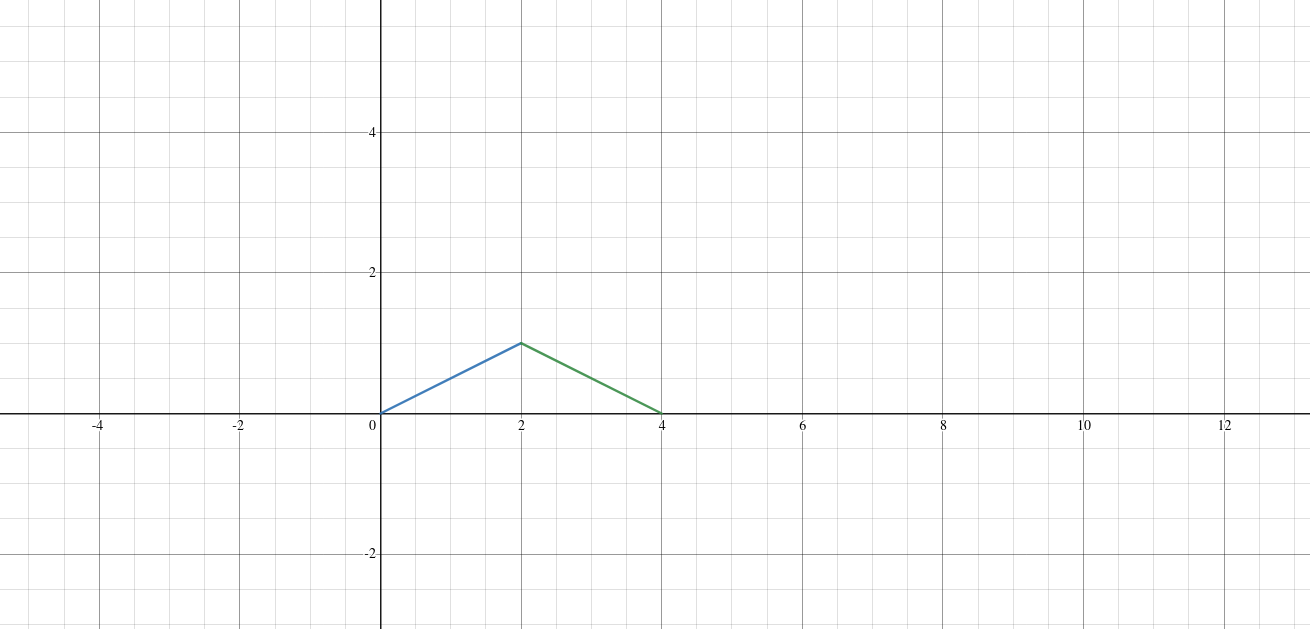
\includegraphics[width=0.8\textwidth]{q3}
    \caption{q3}
    \label{fig:q3}
\end{figure}

{\noindent\bf Question 3b.} To find the wavefunction we must express the initial state as a linear combination of the allowable space dependent solutions, i.e.
\[
\Psi(x, 0)=\sqrt{\frac{2}{a}} \sum_{n=1}^{\infty}c_n\sin\left( \frac{n\pi}{a}x \right) 
.\]
To find the coeefficients $c_n$ we can use fourier's trick: 
\[
c_n=\int\psi_n^*\Psi(x, 0) dx
.\]
To solve this we can use the fact that each of the time independent solutions are symmetric around $\frac{a}{2}$. Since the given initial conditions is also symmetric around 0, all the even terms cancel out with the other half, and means we can just do one integral and assume that the $n$ is odd: 
\[
c_n=2\int_0^{\frac{a}{2}}\sqrt{\frac{2}{a}} \sqrt{\frac{12}{a^3}}x\sin\left( \frac{n\pi}{a}x \right) dx=\frac{4\sqrt{3} }{a^2}\left( \frac{-ax\cos\left( \frac{n\pi}{a}x \right) }{n\pi}\bigg|_0^{\frac{a}{2}} +\int_0^{\frac{a}{2}} \frac{a}{n\pi}\cos\left( \frac{n\pi}{a}x \right)dx \right)
\]
\[
=\frac{4\sqrt{3} }{a^2}\left( \frac{-a^2\cos\left( \frac{n\pi}{2} \right)+a^2 }{2n\pi} +\frac{a^2}{n^2\pi^2}\sin\left( \frac{n\pi}{2} \right)  \right)
\]
\[
=
\begin{cases}
    0&\text{ if $n$ even}\\
    (-1)^{\frac{n-1}2}\frac{4\sqrt{6} }{n^2\pi^2}&\text{ if $n$ odd}
\end{cases}
.\]

Thus the final expression for the time dependent solution is 

\[
\Psi(x, t)=\frac{8}{\pi^2}\sqrt{\frac{3}{a}}\sum_{n\text{ odd}}(-1)^{\frac{n-1}2}\frac{1}{n^2}e^{-in^2\pi^2\hbar t / (2ma^2)}\sin\left( \frac{n\pi}{a}x \right) 
.\]

The probability correspond to the square of the weights $c_n$, so we have that the probability is 
\[
|c_n|^2=\frac{96}{\pi^4}\approx 0.99
.\]

{\noindent\bf Question 3d.} Doing the sum: 

\[
\left<H \right>=\sum_{n\text{ odd}} |c_n|^2 E_n=\sum_{n\text{ odd}}\frac{96 \hbar^2}{2ma^2n^2\pi^2}
.\]
Using the identity that the sum of the odd reciprocal squares is $\frac{\pi^2}{8}$ (similar to the Basel identity), we get 
\[
\left<H \right>=\frac{6\hbar^2}{ma^2}
.\]

{\noindent\bf Question 4.} First note that clearly to normalize the function we have that $A=\sqrt{\frac{2}{a}} $The relative likelyhood of energy states remains constant, so all we have to do is find what $|c_1|$ is. To do so we integrate in a similar way as the last question: 
\[
c_1=\int_0^{\frac{a}{2}}\frac{2}{a}\sin\left( \frac{\pi}{a}x \right) dx=\frac{2}{\pi}
.\]
The probability of the wavefunction being in a particular state when measured is the square of the coefficient corresponding to that state, i.e.
\[
|c_1|^2=\left( \frac{2}{\pi} \right) ^2\approx 0.41
.\]

\end{document}
